\documentclass[
  a4paper,
  12pt,
  spanish,
]{scrartcl}

% Párrafos
\setlength{\parindent}{18pt}
\linespread{1.05}

%-------------------------------------------------------------------------------
%	PAQUETES
%-------------------------------------------------------------------------------

% Idioma

\usepackage[es-noindentfirst, es-tabla]{babel}

% Citas de texto en línea/bloque

\usepackage[autostyle]{csquotes}

% Tablas

\usepackage{booktabs}
\usepackage{multirow}

% Matemáticas

\usepackage{amsmath, amsthm, amssymb}
\usepackage{mathtools}
\usepackage{commath}

% Fuentes personalizadas para utilizar con XeLaTeX o LuaLaTeX

\usepackage[no-math]{fontspec}
\setmainfont{Libertinus Serif}
\setsansfont{Libertinus Sans}
\setmonofont{Libertinus Mono}

\usepackage[math-style=TeX]{unicode-math}
\setmathfont{Libertinus Math}

% Configuración de microtype

\defaultfontfeatures{Ligatures=TeX,Numbers=Lining}
\usepackage[activate={true,nocompatibility},final,tracking=true,factor=1100,stretch=10,shrink=10]{microtype}
\SetTracking{encoding={*}, shape=sc}{0}

% Enlaces y colores

\usepackage{hyperref}
\usepackage[dvipsnames]{xcolor}
\definecolor{webgreen}{rgb}{0,0.5,0}
\hypersetup{
  colorlinks=true,
  citecolor=webgreen,
  urlcolor=Maroon,
  linkcolor=RoyalBlue
}

% Otros elementos de página

\usepackage{enumitem}
\setlist[enumerate]{leftmargin=*, itemsep=0pt}
\setlist[itemize]{leftmargin=*, itemsep=0pt}

\usepackage[labelfont=sc]{caption}
\usepackage[labelfont=default]{subcaption}
%\usepackage{graphicx}

% Tikz

\usepackage{tikz}
\usetikzlibrary{babel}
\usepackage{float}

% Código

\usepackage{listings}
\lstset{
	basicstyle=\footnotesize\ttfamily,%
	breaklines=true,%
	captionpos=b,                    % sets the caption-position to bottom
  tabsize=2,	                   % sets default tabsize to 2 spaces
  frame=lines,
  numbers=left,
  stepnumber=1,
  aboveskip=12pt,
  showstringspaces=false,
}
\renewcommand{\lstlistingname}{Listado}

% Algoritmos

\usepackage[linesnumbered, vlined]{algorithm2e}
\SetAlFnt{\sffamily}
\newcommand{\mykwfont}{\bfseries\sffamily}
\SetKwSty{mykwfont}

\SetKwInput{KwIn}{Entrada}%
\SetKwInput{KwOut}{Salida}%

\SetAlCapSkip{1em}
\SetAlCapFnt{\normalfont\scshape}

% Bibliografía

\usepackage[sorting=none, style=apa, isbn=true]{biblatex}
\DefineBibliographyStrings{spanish}{
  urlseen = {Consultado},
  retrieved = {Consultado},
}
\addbibresource{bibliografia.bib}

% Lorem ipsum

\usepackage{blindtext}

% Márgenes
\usepackage[bottom=3.125cm, top=2.5cm, left=4.5cm, right=4.5cm, marginparwidth=70pt]{geometry}

% Fuentes

\usepackage{textcase}

\newfontfamily{\sacshape}{Libertinus Serif}[
  WordSpace={1.8},
  LetterSpace={18.0}
]

\newfontfamily{\slscshape}{Libertinus Serif}[
  WordSpace={1.8},
  LetterSpace={6.0}
]

\DeclareRobustCommand{\spacedallcaps}[1]{{\linespread{1.3}\sacshape\MakeTextUppercase{#1}}}% WordSpace=1.8
\DeclareRobustCommand{\spacedlowsmallcaps}[1]{{\slscshape\MakeTextLowercase{#1}}}% WordSpace=1.8

% Cabeceras de sección

\RedeclareSectionCommands[beforeskip=-3ex,
afterskip=2ex]{section,subsection,subsubsection}
%\addtokomafont{section}{\normalfont\large\spacedallcaps}
%\setkomafont{section}{\normalfont\large\scshape}
\RedeclareSectionCommand[beforeskip=-9ex, font=\normalfont\large\scshape, tocentryformat=\normalfont\scshape]{section}
\addtokomafont{subsection}{\normalfont\normalsize\itshape}
\RedeclareSectionCommand[beforeskip=-6ex,tocentryformat=\normalfont\itshape]{subsection}
\addtokomafont{subsubsection}{\normalfont}
\RedeclareSectionCommand[beforeskip=-4ex]{subsubsection}
\addtokomafont{paragraph}{\normalfont\itshape}

% Entornos

\newtheoremstyle{teorema-style}  % Nombre del estilo
{1\topsep}                                  % Espacio por encima
{1\topsep}                                  % Espacio por debajo
{\itshape}                                  % Fuente del cuerpo
{0pt}                                  % Identación
{\scshape}                      % Fuente para la cabecera
{.}                                 % Puntuación tras la cabecera
{5pt plus 1pt minus 1pt}                              % Espacio tras la cabecera
{{\thmname{#1}\thmnumber{ #2}}\thmnote{ (#3)}}  % Especificación de la cabecera

\theoremstyle{teorema-style}
\newtheorem*{nth}{Teorema}

%-------------------------------------------------------------------------------
%	TÍTULO
%-------------------------------------------------------------------------------

\newcommand{\horrule}[1]{\rule{\linewidth}{#1}}

%-------------------------------------------------------------------------------
%	CONTENIDO
%-------------------------------------------------------------------------------

\begin{document}

\begin{titlepage}
  \vspace*{4cm}

  \begin{flushleft}
    \Huge
    \spacedallcaps{Redes neuronales artificiales}
    \horrule{2pt}
  \end{flushleft}

  \vspace{2em}

  \begin{flushright}
    \large
    Johanna Capote Robayna\\
    Antonio Coín Castro\\
    Guillermo Galindo Ortuño\\
    José María Martín Luque\\
    Luis Antonio Ortega Andrés\\
    Cristina de la Torre Villaverde
    \vspace{1em}

    \textit{Estadística Multivariante}

    Grado en Matemáticas

    \textsc{Universidad de Granada}\vspace{1em}

    \today\vspace{.5em}
  \end{flushright}
\end{titlepage}

\newpage

{\hypersetup{hidelinks}
\tableofcontents
}

\newpage

\section{Introducción}

\begin{figure}[h]
  \centering
  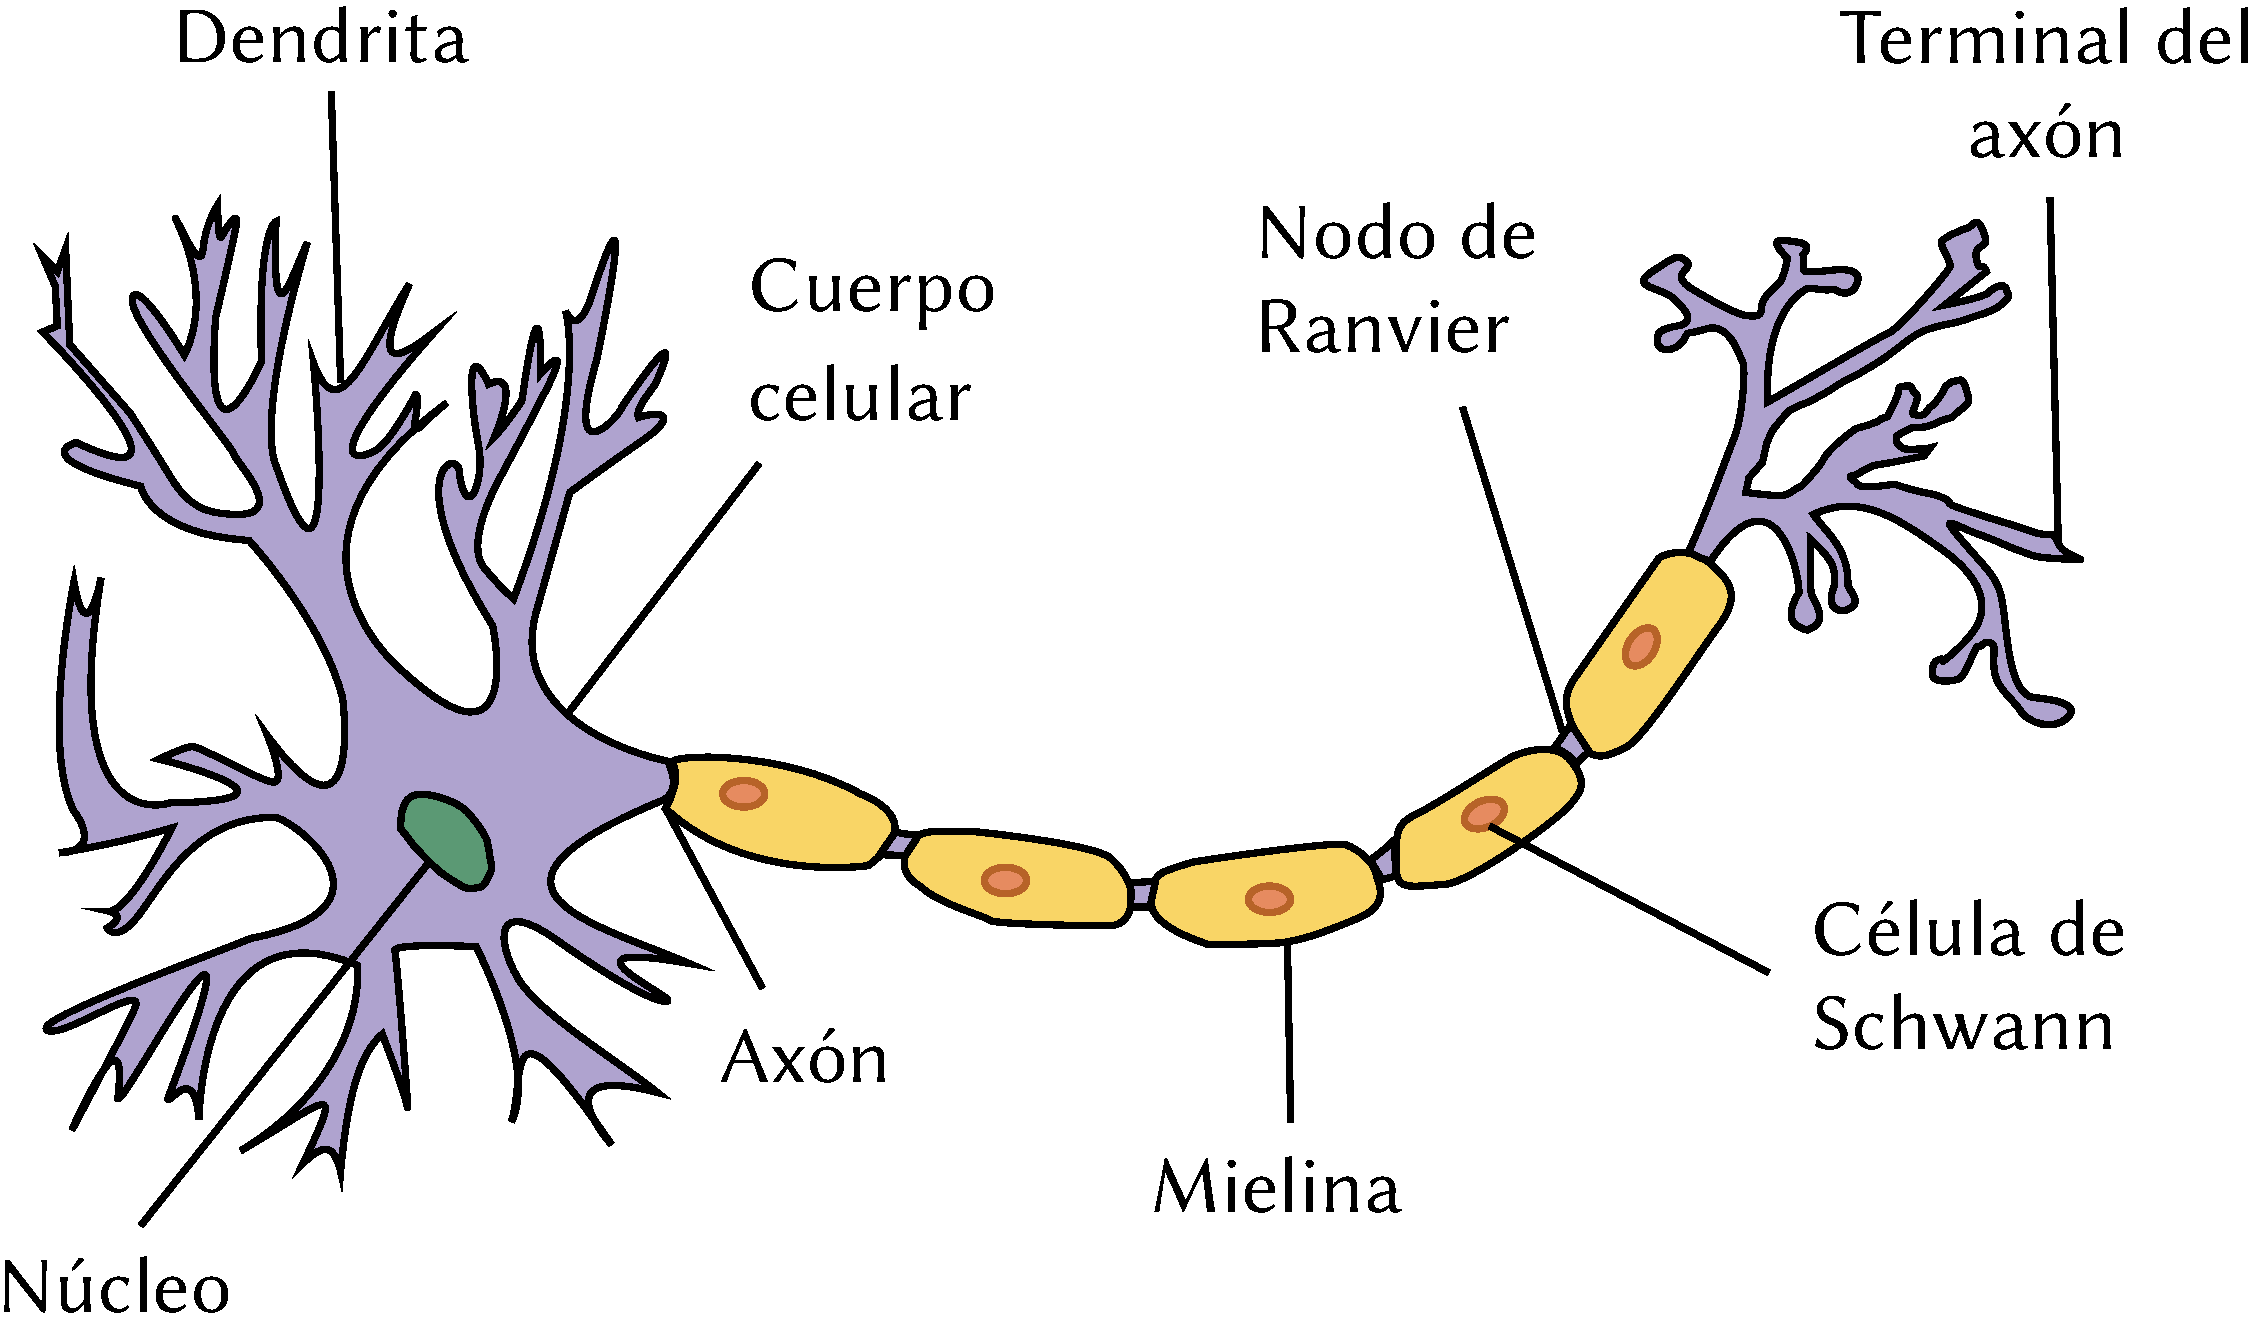
\includegraphics[width=.7\textwidth]{img/neurona}
  \caption{Estructura de una neurona. Basada en \parencite{dhp1080_neurona_2007}.}
  \label{fig:neurona}
\end{figure}


\section{Estructura y funcionamiento de las redes neuronales}

\subsection{La neurona de McCulloch-Pitts}

La neurona de McCulloch-Pitts \parencite{mcculloch_logical_1943} es un modelo computacional que consiste en múltiples entradas (imitando las dendritas) y una sola salida (imitando el axón). Las entradas se denotan por $X_1,X_2,\dots, X_r$ y la salida por $Y$, donde cada una puede tomar el valor $0$ (apagado) o $1$ (activado). Cada conexión puede ser de tipo excitador o inhibidor, y si alguna de ellas es inhibidora y transmite el valor $1$, la salida es directamente $0$. Si no hay conexiones inhibidoras activadas se suman las entradas para producir un valor de \textit{excitación total} $U = \sum_{j} X_j$, y se compara con un valor de \textit{umbral} $\theta$: si $U \ge \theta$ la salida es $Y=1$, en otro caso la salida es $Y=0$. Notamos que si $\theta > r$ la salida siempre será $0$, y si $\theta = 0$ y no hay conexiones inhibidoras activadas, la salida será siempre $1$. Podemos ver una ilustración de esta neurona en la Figura \ref{fig:mcculloch-pitts}.

\begin{figure}[h]
  \centering
  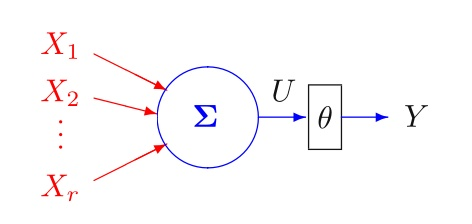
\includegraphics[width=.7\textwidth]{img/mcculloch-pitts}
  \caption{Neurona de McCulloch-Pitts con $r$ entradas binarias $X_1,\dots,X_r$, una salida binaria $Y$ y un umbral $\theta$. Extraída de \parencite{izenman_modern_2008}.}
  \label{fig:mcculloch-pitts}
\end{figure}

Observamos que para un valor fijo de $\theta$, la neurona de McCulloch-Pitts divide el espacio de entrada en dos mitades determinadas por el hiperplano $\sum_j X_j = \theta$; los puntos $(X_1, \dots, X_r)$ con salida $Y=1$ quedan a un lado del hiperplano, mientras que aquellos con $Y=0$ quedan en el otro lado.

A modo de ejemplo, podemos utilizar esta neurona para implementar las funciones lógicas AND y OR de $r$ entradas. Para la función AND elegimos como umbral $\theta = r$, y así la salida tomará el valor 1 únicamente cuando todas las entradas sean 1. Para la función OR elegimos como umbral $\theta = 1$ para que la salida sea $1$ en cuanto alguna de las entradas sea $1$. La construcción de la función NOT es también inmediata, sin más que considerar una única entrada inhibidora y un umbral de $0$, por lo que combinando neuronas de McCulloch-Pitts podemos construir cualquier función booleana.

A pesar de la universalidad mostrada, este modelo no es adecuado para realizar un proceso de aprendizaje, pues la única forma de resolver diferentes problemas es ir cambiando el número y tipo de las entradas y el valor del umbral. Esto hizo que se perdiese rápidamente el interés en este modelo computacional.

\subsection{Perceptrón de una capa}

A principios de los años 60 se produjo una segunda oleada de interés en las redes neuronales artificales, cuando el psicólogo Frank Rosenblatt desarrolló un sistema llamado \textit{perceptrón} \parencite{rosenblatt_perceptron_1958} para imitar el funcionamiento de una neurona. Se trata básicamente de una neurona de McCulloch-Pitts dotada de unos \textit{pesos} $\beta_i \in \mathbb{R}$ en cada conexión $i=1,2,\dots, r$. Los pesos positivos representan conexiones excitadoras, los pesos negativos conexiones inhibidoras y la magnitud de los mismos muestra la fuerza de la conexión.

En este caso, se calcula la suma ponderada $U=\sum_j \beta_j X_j$, y la neurona se activa únicamente si $U\ge \theta$. Podemos convertir el umbral a $0$ introduciendo un elemento de \textit{sesgo} $\beta_0 = -\theta$ y una nueva pseudovariable $X_0 = 1$. De esta forma, como $U-\theta = \beta_0 + U$, podemos simplemente comparar $U=\sum_{j=0}^r \beta_j X_j$ con $0$. En la Figura \ref{fig:perceptron} podemos ver un esquema de un perceptrón descrito de esta forma.

\begin{figure}[h]
  \centering
  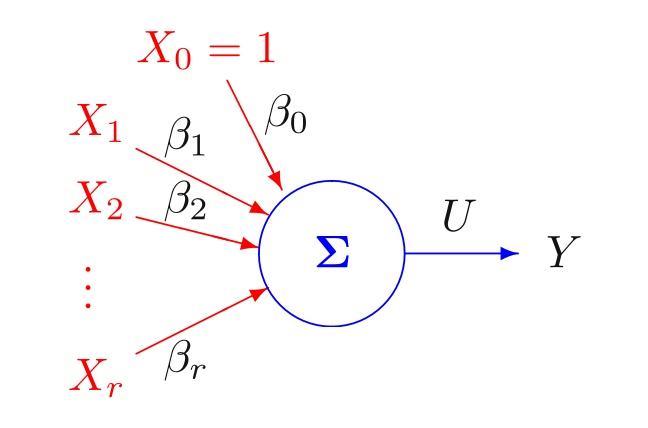
\includegraphics[width=.7\textwidth]{img/perceptron}
  \caption{Perceptrón de $r$ entradas binarias con pesos $\{\beta_j\}$ y salida binaria $Y$. Incluye el término de sesgo $\beta_0$. Extraída de \parencite{izenman_modern_2008}.}
  \label{fig:perceptron}
\end{figure}

Si los datos de entrada son \textit{linealmente separables} (es decir, se pueden separar por un hiperplano), podemos interpretar un perceptrón como un algoritmo de \textit{clasificación binaria}, de forma que los puntos con $Y=0$ pertenecen a una clase distinta a la de aquellos con $Y=1$; la partición queda determinada por el hiperplano $U=\theta$. Sin embargo, si los datos de entradan no son linealmente separables, la función $Y$ asociada no es computable por un perceptrón (un ejemplo de este caso es la función XOR). En la Figura \ref{fig:separable} puede verse una representación gráfica de datos separables y no separables linealmente.

\begin{figure}[h]
  \centering
  \begin{subfigure}[b]{0.4\textwidth}
    \centering
    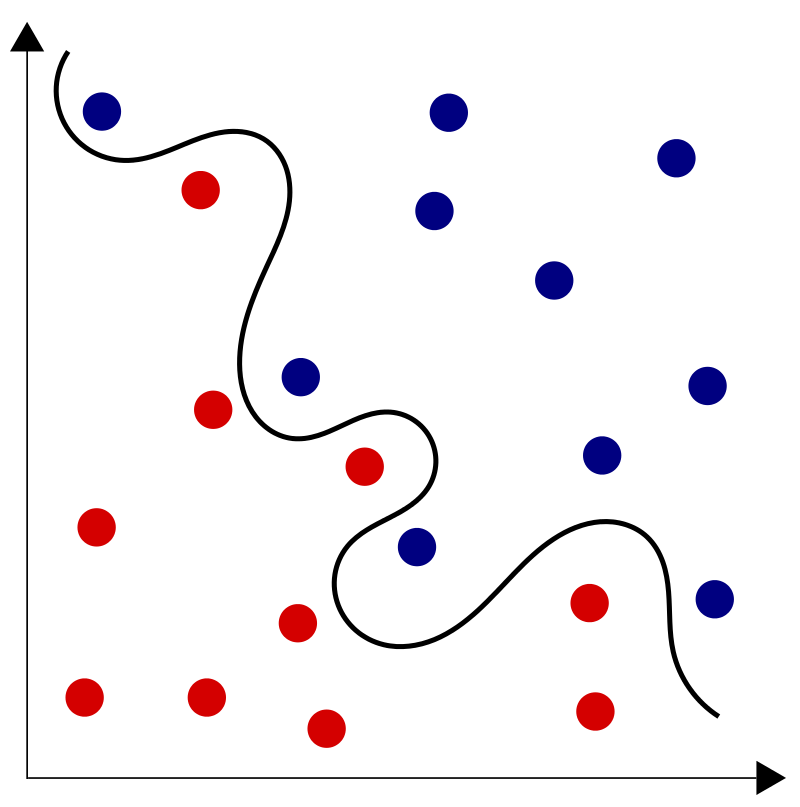
\includegraphics[width=.8\textwidth]{img/non-separable}
    \caption{No linealmente separables}
  \end{subfigure}
  \qquad
  \begin{subfigure}[b]{0.4\textwidth}
    \centering
    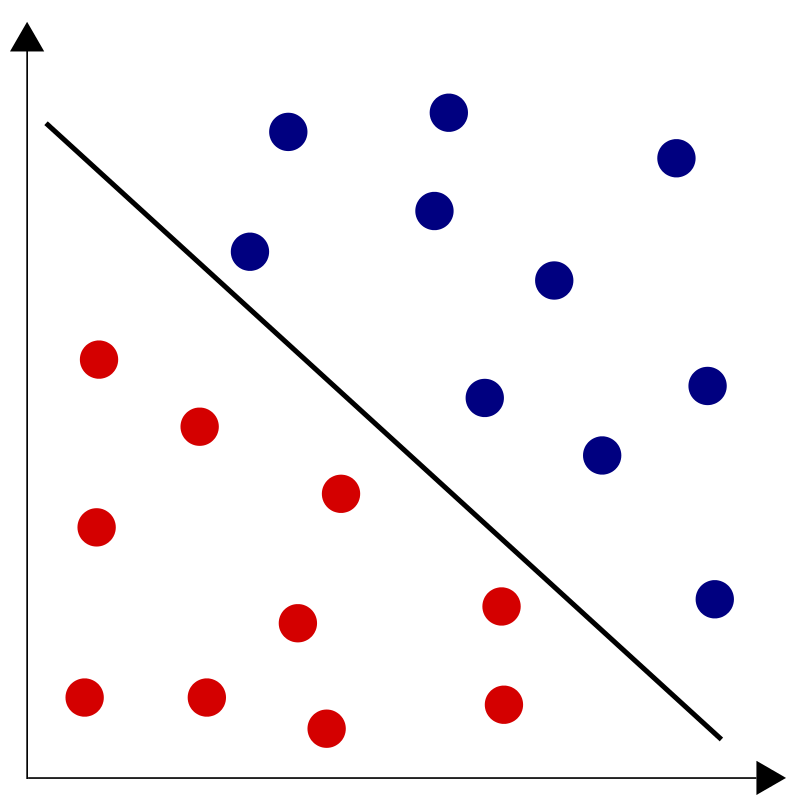
\includegraphics[width=.8\textwidth]{img/separable}
    \caption{Linealmente separables}
  \end{subfigure}
  \caption{Ejemplos de datos bidimensionales separables y no separables linealmente. Extraída de \parencite{wikipedia_separable}.}
  \label{fig:separable}
\end{figure}

Podemos considerar una red neuronal de perceptrones interconectados organizados en dos grupos: $r$ nodos de entrada $\{X_j\}$ y $s$ nodos de salida $\{Y_k\}$, que pueden tomar tanto valores reales como discretos. Cada conexión $X_j \to Y_k$ está marcada por un peso $\beta_{jk}$. Este tipo de redes se conocen como \textit{redes de una capa}, pues aunque hay dos grupos solo se realizan cálculos significativos en los nodos de salida.

\subsection{Funciones de activación}

El objetivo ahora es construir una red de una capa que dado un problema sea capaz de aprender unos pesos para resolverlo. No es difícil darse cuenta de que hasta ahora en cada perceptrón solo hemos computado una transformación afín de los datos de entrada: si $\mathbf{X}=(X_1, \dots, X_r)^T$ es un vector aleatorio de entradas y tenemos $s$ nodos de salida, en cada uno de ellos calculamos
\[
U_k = \beta_{0k} + \mathbf{X}^T \pmb\beta_k, \quad k = 1,\dots, s,
\]
donde $\beta_{0k}$ es la constante de \textit{sesgo} y $\pmb{\beta}_k = (\beta_{1k}, \dots, \beta_{rk})^T$ es un vector de pesos. De esta forma la red no podría aprender funciones que tengan un comportamiento no lineal, y es por esto que se introduce el concepto de \textit{función de activación}. Consideramos una función no lineal $f$ que se aplica a la salida de cada nodo, de forma que la salida final obtenida es
\[
U_k = f(\beta_{0k} + \mathbf{X}^T \pmb{\beta}_k), \quad k = 1,\dots, s.
\]

Ejemplos de funciones de activación comunes son \textit{sigmoides} como la función logística o la tangente hiperbólica, y también la función \textit{signo} para problemas de clasificación binaria. En los últimos años se ha popularizado el uso de la función ReLU dada por $f(x) = x^+ = \max{\{0, x\}}$, cuya gráfica podemos ver en la Figura \ref{fig:relu}.

\begin{figure}[h]
  \centering
  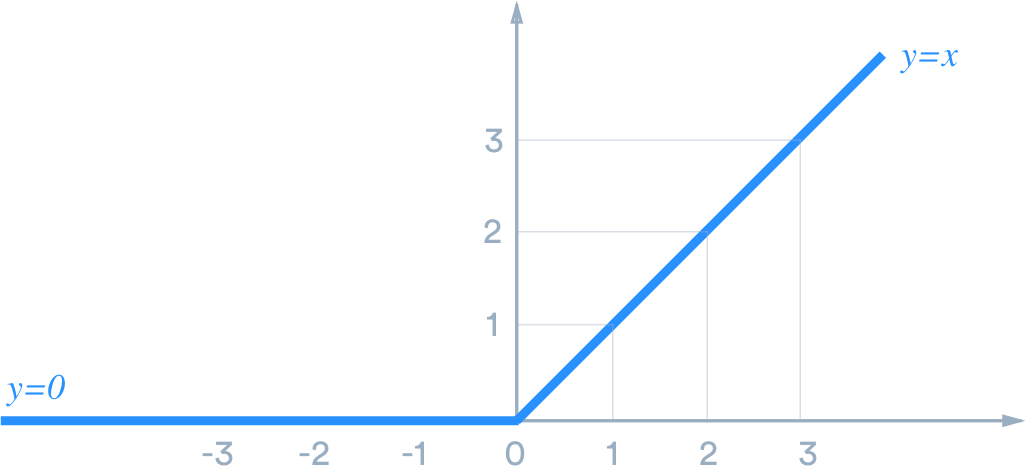
\includegraphics[width=.7\textwidth]{img/relu}
  \caption{Gráfica de la función ReLU.}
  \label{fig:relu}
\end{figure}

En el contexto de problemas de \textit{clasificación multiclase} podemos considerar también una función de activación vectorial $\pmb f$ aplicada al vector de \textit{outputs} $\pmb U = (U_1, \dots, U_s)^T$. Por ejemplo, la función \textit{softmax} $\pmb f(\pmb x)_i = e^{x_i}/\sum_{k=1}^s e^{x_k}$ se puede entender como una distribución de probabilidad en $s$ valores, de forma que la salida en el nodo $k$-ésimo representa la probabilidad de pertenecer a la $k$-ésima clase.

\subsection{Proceso de aprendizaje}

La clave del funcionamiento de esta arquitectura es que se puede definir un proceso iterativo mediante el cual la red es capaz de \textit{aprender} los pesos óptimos para resolver un problema de clasificación binaria. Suponemos que tenemos una serie de ejemplos de entrada independientes $\pmb X_1, \dots, \pmb X_n$ extraídos de dos clases $\Pi_1$ y $\Pi_2$, y un único nodo de salida. Incorporando el valor del sesgo al vector de pesos y adoptando la notación $\pmb \beta \leftarrow (\beta_0, \pmb \beta^T)^T$ y $\pmb X \leftarrow (1, \pmb X^T)^T$, podemos reescribir $\beta_{0} + \mathbf{X}^T \pmb{\beta}$ como $\mathbf{X}^T \pmb{\beta}$. Para un estado concreto de la red (es decir, unos pesos fijos $\pmb \beta$), interpretaremos que un ejemplo $\pmb X$ pertenece a la primera clase si y solo si $\pmb X^T \pmb \beta \ge 0$. La estrategia es utilizar el conocimiento de la clase correcta para ir pasando los ejemplos por la red y predecir la clase a la que pertenece cada uno, intentando corregir los pesos si se detecta un error. Esta técnica se conoce como \textit{aprendizaje supervisado}.

La regla para actualizar los pesos en cada iteración es la siguiente:
\begin{enumerate}
  \item Si la versión actual de los pesos $\pmb \beta_h$ consigue clasificar correctamente $\pmb X_h$, no cambiamos los pesos para la siguiente iteración.
  \item Si con los pesos $\pmb \beta_h$ no obtenemos una clasificación correcta, hacemos
\[
  \pmb \beta_{h+1} = \pmb \beta_h + \eta \operatorname{signo}(\pmb X^T_h \pmb \beta_h) \pmb X_h.
\]
El parámetro $\eta > 0$ se conoce como \textit{learning rate}, y controla en qué proporción varían los pesos en cada iteración.
\end{enumerate}

Una solución del problema será un vector de pesos $\pmb \beta^\ast$ que clasifique correctamente todos los ejemplos, es decir, que todos los que estén a un mismo lado del hiperplano $\pmb X_h^T \pmb \beta^\ast$ pertenezcan a la misma clase. Para esto es necesario que los datos de entrada sean linealmente separables. La utilización de este método se justifica gracias al siguiente resultado.

\begin{nth}[Convergencia del perceptrón]
Para un problema de clasificación binaria con clases linealmente separables, si existe una solución $\pmb \beta^\ast$, el algoritmo descrito anteriormente la encontrará en un número finito de iteraciones.
\end{nth}

Este algoritmo se puede extender a problemas de clasificación multiclase. Dada una \textit{función de error} diferenciable $F(\pmb x)$ que mida la diferencia entre la clase predicha y la clase real, se utiliza un algoritmo de \textit{gradiente descendente} que propaga hacia atrás el error en cada iteración y modifica los pesos de acuerdo a la regla
\[
\pmb \beta_{h+1} = \pmb \beta_h - \eta \nabla F_h(\pmb \beta_h).
\]
Notamos que perseguimos minimizar la función de error avanzando en la dirección y sentido de máxima pendiente: la que marca el gradiente cambiado de signo.

\subsection{Perceptrón multicapa}

A mediados de los años 80 se acuñó finalmente el concepto de \textit{perceptrón multicapa}. Se trata de un modelo que pretende solventar las limitaciones del perceptrón distribuyendo los nodos en varias capas y aplicando transformaciones no lineales en el paso de una capa a la siguiente. Las capas intermedias se conocen como \textit{capas ocultas}. Podemos ver un esquema de este modelo en la Figura \ref{fig:multi}.

\begin{figure}[h]
  \centering
  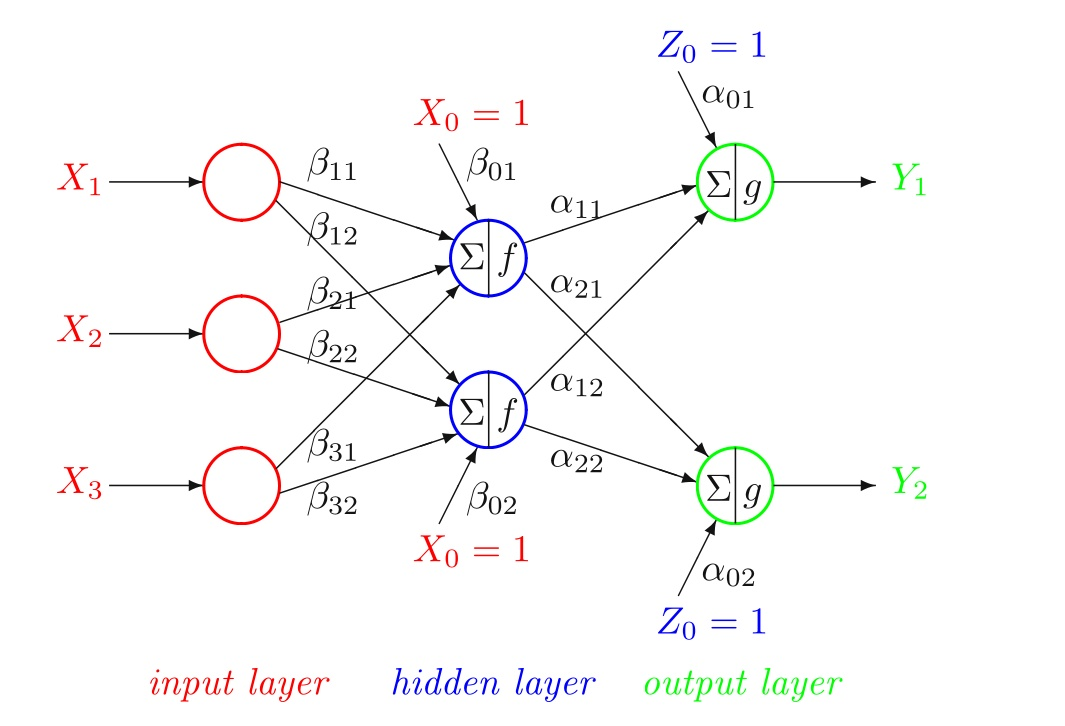
\includegraphics[width=.8\textwidth]{img/multicapa}
  \caption{Esquema de un perceptrón multicapa totalmente conectado con una capa oculta.}
  \label{fig:multi}
\end{figure}

En general, una red con $L$ capas ocultas se conoce como una red de $L+1$ capas (de nuevo, la capa de entrada no cuenta). Decimos que una capa está \textit{totalmente conectada} cuando todos sus nodos reciben como entrada activaciones de todas las neuronas de la capa anterior, y \textit{parcialmente conectada} en otro caso.

Para el proceso de aprendizaje de la red, se utiliza de nuevo la técnica de gradiente descendente, pero esta vez se va propagando hacia atrás el error en todas las capas, alterando todos los pesos en el proceso de forma iterativa.

Una vez que tenemos unos pesos \textit{suficientemente buenos}, podemos utilizar la red entrenada para clasificar nuevos ejemplos no etiquetados que no ha visto antes, aspirando así a resolver el problema de clasificación en todo el espacio de entrada. La bondad o \textit{precisión} de la red se medirá, dado un conjunto de \textit{test} con nuevos ejemplo, contando el número de de ellos que ha sido capaz de clasificar correctamente.

También podemos abordar el problema de regresión lineal mediante redes neuronales. En particular, si consideramos una red con un único nodo de salida y que utilice únicamente funciones de activación lineal, podremos entrenarla para que aprenda los pesos (coeficientes) de la función lineal que mejor aproxima los datos de entrada. Si utilizamos como función de error el error cuadrático, estaríamos ante una regresión por mínimos cuadrados.

Un punto en contra de los modelos basados en redes neuronales es que sufren de \textit{pérdida de interpretabilidad} frente a modelos clásicos. A cambio, las redes neuronales consiguen resolver problemas mucho más complejos de forma automática, en parte gracias a la gran capacidad de cómputo de la que disponen los ordenadores hoy en día.

\section{Relación con la estadística}

Una de las interpretaciones estadísticas más obvias del Perceptrón multicapa, es que este proporciona una regresión no lineal estimada optimizando en cierta medida los datos de entrenamiento. Si estos últimos no tienen ruido, entonces el ejercicio es de aproximación de funciones. Hay muchos desarrollos sistemáticos recientes en regresión, y se deben enfrentar al menos tres preguntas importantes:
\begin{itemize}
\item ¿Cómo se comparan las redes neuronales y las prescripciones estadísticas en términos de rendimiento?
\item ¿Como de buenas son las diversas arquitecturas a la hora de aproximar miembros de clases particulares de funciones de regresión?
\item ¿Cuáles son los métodos numéricos más confiables y prácticos para la estimación de parámetros?
\end{itemize}

El Perceptrón de una capa y el Perceptrón multicapa definen dos de los desarrollos estadísticos: la regresión de búsqueda-proyección y los modelos aditivos generalizados.

El problema de encontrar pesos óptimos para un asociador lineal y para un
El conjunto de entrenamiento dado $T$ se conoce en estadística como regresión lineal múltiple. Estamos
buscando constantes $w_0, w_1, \cdots w_n$ tal que los valores y se puedan calcular
de los valores $x$:
$$y_i = w_0 + w_1 x_1^i + w_2 x_2^i + \cdots + w_n x_n^i + \epsilon_i $$
donde $\epsilon_i$ representa la aproximación del error (notamos que no hemos incluido la constante $w_0$ en la aproximación). Las constantes seleccionadas deben minimizar el error cuadrático $\sum_{i=1}^{n} \epsilon_i^2$. Este problema se puede resolver utilizando métodos algebraicos. (Introducir o no la resolucion algebraica???? Pag 4 de Statistics and NN )


%-------------------------------------------------------------------------------
%	BIBLIOGRAFÍA
%-------------------------------------------------------------------------------

\newpage
\printbibliography

\end{document}
